\documentclass[addpoints]{exam}

%\printanswers
\noprintanswers

\usepackage{amsmath,bigstrut,minted,url,graphicx,tikz,tikz-qtree}

\pagestyle{headandfoot}
\runningheadrule
\firstpageheader{}{}{Page \thepage\ of \numpages}
\runningheader{CS 321}{Sample Problems}{Page \thepage\ of \numpages}
\firstpagefooter{}{}{}
\runningfooter{}{}{}
              
\begin{document}

\begin{center}
{\Large \textbf{
    Ozyegin University\\
    CS 321 Programming Languages\\
    Sample Problems on Interpretation
}}
\end{center}

\begin{questions}
  \question
  (From PLC, Exercise 1.1)
  Given the definition of the simple ArithLang below,
  extend this language with conditional expressions (i.e. ``if'')
  corresponding to Java's expression \texttt{$e_1$ ? $e_2$ : $e_3$},
  or OCaml's \texttt{if $e_1$ then $e_2$ else $e_3$}.
  Evaluation of a conditional expression should evaluate $e_1$ first.
  If it yields a non-zero value, evaluate $e_2$, otherwise evaluate $e_3$.
  
  \inputminted{ocaml}{arith.ml}

  \begin{solutionbox}{9cm}
    Here is the diff:
    \inputminted{diff}{arith_if_diff.txt}
  \end{solutionbox}


  \newpage
  \question
  (From PLC, Exercise 1.1)
  Extend ArithLang to handle three additional operators:
  ``max'', ``min'', and ``=''.
  Like the existing binary operators,
  they take two argument expressions.
  The equals operator should return 1 when true and 0 when false.

  \begin{solutionbox}{14cm}
    Here is the diff:
    \inputminted{diff}{arith_minmaxeq_diff.txt}
  \end{solutionbox}

  
  \question
  Write the representation of the following ArithLang expressions
  using the \texttt{exp} data type.
  \begin{parts}
    \part \mintinline{ocaml}{v * 5 - k + 6}
    \begin{solutionbox}{1cm}
      \mintinline{ocaml}{Add(Subt(Mult(Var "v", CstI 5), Var "k"), CstI 6)}
    \end{solutionbox}
    
    \part \mintinline{ocaml}{x + y + z + p}
    \begin{solutionbox}{1cm}
      \mintinline{ocaml}{Add(Add(Add(Var "x", Var "y"), Var "z"), Var "p")}
    \end{solutionbox}
    
    \part \mintinline{ocaml}{5 - (y - 3) * (g + 1)}
    \begin{solutionbox}{1cm}
      \mintinline{ocaml}{Subt(CstI 5, Mult(Subt(Var "y", CstI 3), Add(Var "g", CstI 1)))}
    \end{solutionbox}  

    \part
    \begin{minted}{ocaml}
    let x =
      let a = 5
      in let b = 8
         in a + b
    in x * (let y = x + 2 in y)
    \end{minted}
    \begin{solutionbox}{4cm}
      \begin{minted}{ocaml}
        LetIn("x",
              LetIn("a", CstI 5,
                    LetIn("b", CstI 8,
                          Add(Var "a", Var "b"))),
              Mult(Var "x",
                   LetIn("y", Add(Var "x", CstI 2),
                         Var "y"))) 
      \end{minted}
    \end{solutionbox}  
\end{parts}


  \question
  Write an OCaml function named \texttt{simplify}
  that takes an \texttt{exp} and returns its simplified form
  based on the rules below:

  {
    \begin{center}
    \begin{tabular}{c}\hline
      $0+e \to e$\\
      $e+0 \to e$\\
      $e-0 \to e$\\
      $1\times e \to e$\\
      $e\times 1 \to e$\\
      $0\times e \to 0$\\
      $e\times 0 \to 0$\\
      $e-e \to 0$\\\hline
    \end{tabular}
    \end{center}
  }

  Remark: This problem is harder than it seems, because
  simplification of expressions may enable other simplifications,
  and I want to you to handle those cases, too.   
  See the test cases.

  \begin{minted}{ocaml}
    # simplify (Mult(CstI 1,
                     Mult(Add(Add(CstI 1,
                                  Subt(Var "x", Var "x")),
                              Add(CstI 4, CstI 6)),
                          CstI 1)));;
    - : exp = Add(CstI 1, Add(CstI 4, CstI 6))
    
    # simplify (Subt(CstI 0, Mult(Add(Var "x", CstI 0), CstI 0)));;
    - : exp = CstI 0
    
    # simplify (LetIn("a", CstI 4,
                      Subt(CstI 0,
                           Mult(Add(Var "x", CstI 0),
                                CstI 0))));;
    - : exp = LetIn("a", CstI 4, CstI 0)

    # simplify (Subt(Add(CstI 7, CstI 0),
                     Mult(Add(Var "x", CstI 0), CstI 0)));;
    - : exp = CstI 7

    # simplify (Div(Subt(CstI 0,
                         Mult(Add(Var "x", CstI 0), CstI 0)),
                    CstI 7));;
    - : exp = Div(CstI 0, CstI 7)
  \end{minted}

  \begin{solutionbox}{11cm}
    \inputminted{ocaml}{simplify.ml}
  \end{solutionbox}

  \question
  Is the grammar shown below ambiguous?
  If yes, give me an input that at least two different
  parse trees, and show those trees.
  If no, prove it.

  \begin{minted}{ocaml}
    main ::= exp EOF
    exp  ::= INT
           | NAME
           | exp PLUS exp
           | exp STAR exp
           | LET NAME EQ exp IN exp
           | IF exp THEN exp ELSE exp
  \end{minted}

  \begin{solutionbox}{12cm}
    It is ambiguous. Here is an input:
    \mintinline{ocaml}{let x = 5 in x + 9}.

    \Tree[.main
      [.exp
        LET
        {NAME(``x'')}
        EQ
        [.exp {INT(5)} ]
        IN
        [.exp
          [.exp {NAME(``x'')} ]
          PLUS
          [.exp {INT(9)} ]
        ]
      ]
      EOF
    ]
    
    And the second tree is
        
    \Tree[.main
      [.exp
        [.exp
          LET
          {NAME(``x'')}
          EQ
          [.exp {INT(5)} ]
          IN
          [.exp {NAME(``x'')} ]
        ]
        PLUS
        [.exp {INT(9)} ]
      ]
      EOF
    ]
  \end{solutionbox}

  \question
  \begin{minted}{ocaml}
    main ::= exp EOF
    exp  ::= INT
           | NAME
           | exp SLASH exp
           | exp PLUS exp
           | LET NAME EQ exp IN exp
           | IF exp THEN exp ELSE exp
  \end{minted}
  Based on the grammar given above,
  show two different parse trees for the following inputs.
  For each, also state whether the ambiguity is related to
  \textbf{precedence} or \textbf{associativity}.
  \begin{parts}
    \part \mintinline{ocaml}{9 + 5 + 2}
    \begin{solutionbox}{6.5cm}
      This is related to associativity.
      Does the ``+'' sign associate to the left or to the right? That's the problem.
      If ``+'' associates to the right, we would get the tree on the left;
      if ``+'' associates to the left, we would get the tree on the right.

      {\small
      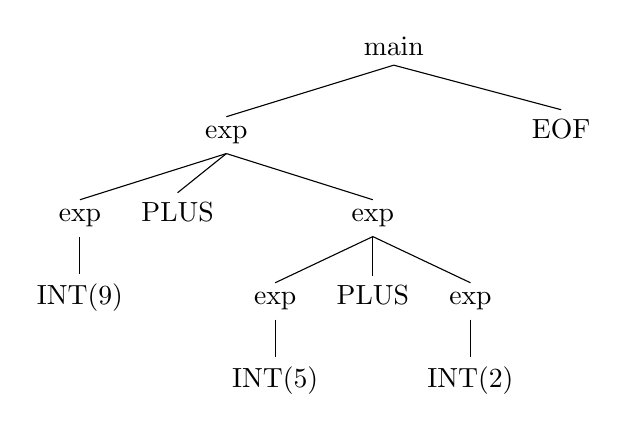
\begin{tikzpicture}[sibling distance=0pt]
        \Tree[.main
        [.exp
          [.exp INT\\(9) ]
          PLUS
          [.exp
            [.exp {INT(5)} ]
            PLUS
            [.exp {INT(2)} ]
          ]
        ]
        EOF
      ]
      \end{tikzpicture}
      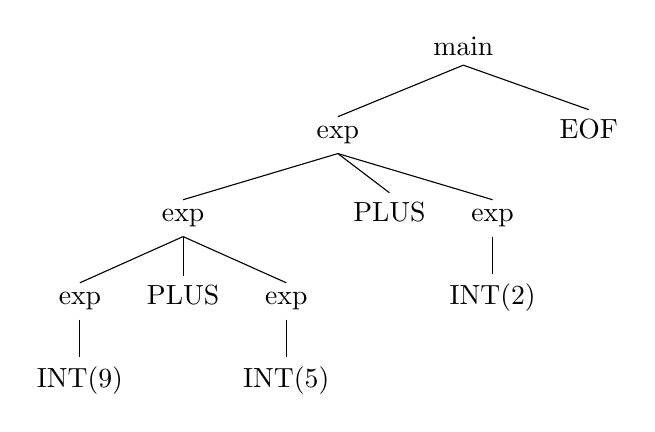
\begin{tikzpicture}
      \Tree[.main
        [.exp
          [.exp
            [.exp {INT(9)} ]
            PLUS
            [.exp {INT(5)} ]
          ]
          PLUS
          [.exp {INT(2)} ]
        ]
        EOF
      ]
      \end{tikzpicture}
      }
    \end{solutionbox}
    
    \part \mintinline{ocaml}{9 + 5 / 2}
    \begin{solutionbox}{7cm}
      This is related to precedence.
      Which operator has higher precedence, ``/'' or ``+''?
      That is, who wins the fight over the ownership of ``5''?
      That's the problem.
      If ``/'' has higher precedence, we would get the tree on the left;
      if ``+'' has higher precedence, we would get the tree on the right.

      {\small
      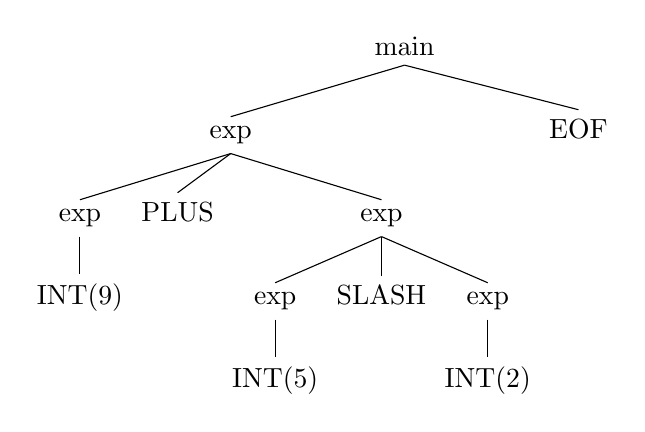
\begin{tikzpicture}[sibling distance=0pt]
        \Tree[.main
        [.exp
          [.exp INT\\(9) ]
          PLUS
          [.exp
            [.exp {INT(5)} ]
            SLASH
            [.exp {INT(2)} ]
          ]
        ]
        EOF
      ]
      \end{tikzpicture}
      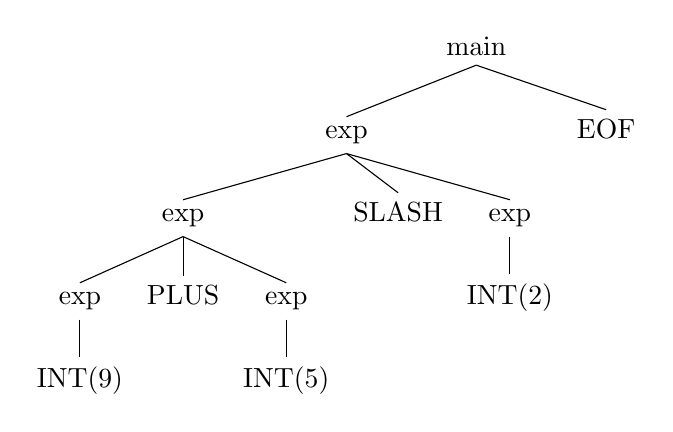
\begin{tikzpicture}
      \Tree[.main
        [.exp
          [.exp
            [.exp {INT(9)} ]
            PLUS
            [.exp {INT(5)} ]
          ]
          SLASH
          [.exp {INT(2)} ]
        ]
        EOF
      ]
      \end{tikzpicture}
      }
    \end{solutionbox}
  \end{parts}
  


\end{questions}

\end{document}
